\chapter{Simulation} \label{chapter:simulation}
Previous chapters have introduced the models that are going to be used to model the \acs{WLAN} traffic behavior. In addition, a short presentation of the traffic model that we are going to use for our experiments, studied in \cite{Campus-WLAN} has been addressed. This chapter will introduce the simulation environment and its configuration and will serve as an introduction to the experiments that follow this section.

As it has been introduced previously, the experiments will be run over the Network Simulation 2 software and its NS-Miracle extension \cite{NSMiracle}. In \cite{marcello-thesis}, the implementation of the previously introduced models for modeling the traffic and the multi-layer traffic model have already been developed.

Our work in this project will mainly test the efficiency of these models and its implementation and, if necessary, we will modify/extend the implementations.

In this chapter we will present briefly the simulation environment. For an extended view of the simulation environment see the implementation defined in \cite{marcello-thesis} and the simulation files provided with this project.

\section{Network Simulation 2} \label{sec:NS}
\acs{NS} is a open-source discrete event simulator of networks that provides support for \acs{TCP}, routing and multicast protocols over wired and wireless networks.

The extension NS-Miracle, is an open-source project that provides a set of libraries of network protocols to fulfill the already implemented in NS2. In addition enables the coexistence of multiple modules in each layer of the protocol stack: multiple IP, link layers, MACs, PHY and so on. NS-Miracle extends the implementation of modern communication systems over NS2. The main library that is going to be used for this project is "dei80211mr", which provides an implementation of the 802.11 protocol over NS2.

In \cite{marcello-thesis} the presented semi-Markovian models and the multi-layer traffic model \cite{Campus-WLAN} have been implemented. The protocol stacks for the \acs{WLAN} and \acs{WSN} have been also implemented as it is presented in Figure \ref{fig:protocol_stack}.

\begin{figure}[h]
	\centering
	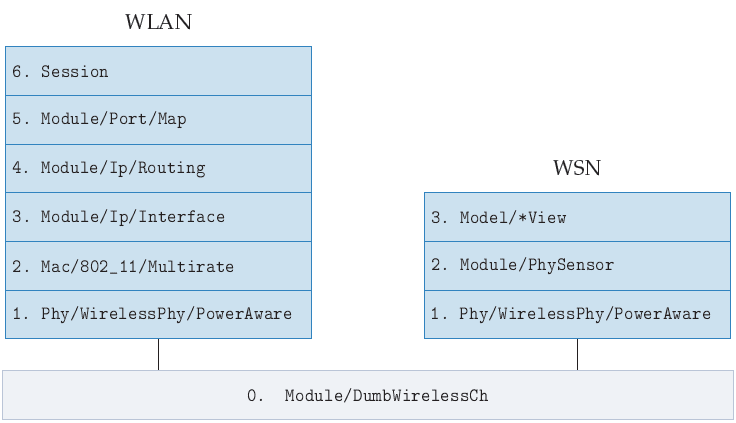
\includegraphics[scale=0.5]{images/simulation/protocol_stack}
	\caption{Protocol stacks for \acs{WLAN} and \acs{WSN} \cite{marcello-thesis}}
	\label{fig:protocol_stack}
\end{figure}

As it can be observed in Figure \ref{fig:protocol_stack}, the protocol stack for the \acs{WSN} is much simpler than the \acs{WLAN}. The sensor will observe the channel using the physical layer implemented in Module 1. The frame will continue to the next layers if it is above the sensing threshold. Module 2 will process the frame, deciding whether or not is a \acs{WSN} or \acs{WLAN} frame, drop, etc. Finally, the third module is the responsible for the estimation process already described in Chapter \ref{chapter:model}.

\section{Traffic generator} \label{sec:traffic_simulation}
As it has been already introduced in Chapter \ref{chapter:traffic_model}, the multi-layer traffic model presented in \cite{Campus-WLAN} has been implemented over the NS2 software, more specifically, a C++ library of random distributions defined in Chapter \ref{chapter:traffic_model}. The traffic will be generated randomly following the distributions defined in \ref{chapter:traffic_model} and using the \acs{GSL} library.

The bi-Pareto distribution is used in the mixture-idle, for this, is composed by a Uniform and a generalized Pareto distributions.

Each one of the distributions can be configured manually choosing the desired parameters via the TCL configuration files provided with the implementation.

\section{Estimation Library} \label{sec:simulation_estimation}
The estimation library is implemented in C++ and comprises different modules that define the estimation processes for the Global and Local View models.

The samples are gathered using the "PhySensor" class. This class manages the samples gathered from the network's traffic, decides whether or not is sensed by the sensor in which the PhySensor class is attached using the specified sensing threshold. Decides if the frame is a \acs{WLAN} or \acs{WSN} communication and which type in case is a \acs{WLAN} frame (\acs{ACK}, \acs{RTS}, \acs{CTS}, data, etc.). And finally adds the idle-active duration for the estimation process.

The estimation library is composed by the following modules that will perform the estimation on the idle samples gathered previously by the PhySensor class:

\begin{itemize}
	\item ModelView: super-class that defines the skeleton for the rest of the estimation modules.
	\item ModelGlobalView: class that defines the estimation processes for the Global View model. It uses the \acs{MLE} estimation process. It returns the estimation parameters for the active and idle distributions.
	\item ModelKSGlobalView: extends the estimation process defined in ModelGlobalView with the Kolmogorov-Smirnov test, which validates the fitting between the empirical and estimated distributions. It returns the D and P values for the \acs{K-S} test in addition to the active and idle distribution parameters.
	\item ModelLocalView: class that defines the estimation processes for the Local View model. It uses the Laplace estimator presented in Section \ref{sec:laplace_estimator}.  It returns the estimation paramters for the active and idle distributions.
	\item ModelKSLocalView: same functionality as the ModelKSGlobalView module but for the Local View model.
\end{itemize}


\section{Validation Test} \label{sec:simulation_validation}
The implementation developed in \cite{marcello-thesis} includes a validation test that will test the fitting between the empirical and estimated distributions.

The validation test will be performed on the truncated part of the mixture idle distribution defined in \ref{eq:Idle}. First of all, the validation test will gather the idle samples. For a faster search of the D and P values, only a 10\% of the idle samples gathered will be used in the validation test\footnote{In the results chapter, we will see how this decision will affect the \acs{K-S} performance.}.

Secondly, obtain the CDF of the samples and find the maximum deviation between both empirical and estimated distributions. The P-value will be determined by comparing the obtained D-value with the D value from a series of uniformly distributed values.

The pseudo-code for this process is presented below even so, there are other possible methods to obtain the p-value for the \acs{K-S} validation test.

\begin{algorithm}
\label{code:laplace}
\begin{algorithmic}
	\item[1] Add idle samples only if $t_{sample} > alpha_{BK}$
	\item[2] Find the maximum deviation between the empirical and estimated distributions
		\hspace{1.5em} \For {$i$ in {$1..num_samples$}} \\
			\hspace{1.5em} Find CDF of sample $i$. \\
			\hspace{1.5em} $d = max(abs(CDF_{empirical} - CDF_{estimated}), d)$
		\EndFor
	\item[3] Estimate the P-value.
		\hspace{1.5em} \For {$i$ in {$1..num_runs$}} \\
			\hspace{1.5em} Generate $N = num_samples$ uniformly distributed values. \\
			\hspace{1.5em} $D = max(abs(CDF_{uniform} - CDF_{estimated}), D)$
			\If {D >= d} \\
				\hspace{1.5em} $count++$
			\EndIf
		\EndFor
	\item[4] Return D and P values. \\
		$P = count/\#runs$.				
\end{algorithmic}
\end{algorithm}

\section{Simulation configuration} \label{sec:simulation_configuration}
In order to define the simulation environment, a TCL library is provided with the \cite{marcello-thesis} implementation. The simulation environment is started using TCL configuration files in which the different layers of the network and other characteristics are specified.

First of all, the environment configuration is needed. The "init.tcl" configuration file includes a list of the different sub-configuration files that define the characteristics of the network environment.

The traffic generation is defined configuring the random distributions presented in Section \ref{sec:traffic_simulation}. The simulation time and other parameters as logs, traffic statistics and so on can also be defined.

Then, the \acs{WLAN} and \acs{WSN} nodes are deployed uniformly distributed or manually in the scenario. Each one of the \acs{WLAN} nodes is linked to another node or an access point. These nodes will generate the traffic accordingly to the multi-layer traffic configuration defined.

The sensing capabilities of the \acs{WSN} nodes need to be defined also in the TCL simulation file. Here, the sensing modules defined in Section \ref{sec:simulation_estimation}, sensing time, number of samples to gather, etc. are defined.

Once the entire configuration is completed, the simulator starts the simulation environment loading the configuration defined in the TCL file. The nodes are deployed in the scenario, the session and flows are initialized and a series of packets will be sent between the nodes during the simulation time defined or until all the flows are empty (for each one of the packets, the size of the flow associated to that packet is decreased).

During this simulation time, the \acs{WSN} gathers the samples needed for the estimation process defined in the model associated to the \acs{WSN} node and returns the active and idle distribution parameters.

The following table shows the main configuration files and its characteristics:

\renewcommand{\arraystretch}{1.8}
\begin{table}[h!]
	\begin{center}
		\begin{tabular}{ l | c }
			\textbf{Configuration file} & \textbf{Characteristics} \\ \hline
			utility/init.tcl & \parbox{10cm}{instantiates the configuration files to be loaded}\\ \hline
			utility/simulation.tcl & \parbox{10cm}{initiate/stop simulator with the parameters defined in the simulation file}\\ \hline
			config/global.tcl & \parbox{10cm}{defines the main parameters and log files}\\ \hline
			config/trace.tcl & \parbox{10cm}{defines which layers will be stored in the trace file}\\ \hline
			config/layer\_N.tcl & \parbox{10cm}{defines the parameters for the layer N}	\\ \hline
			config/layer\_5\_wlan/\*.tcl & \parbox{10cm}{configuration files to define the parameters for the multi-layer traffic generator}\\ \hline
			classes/*.tcl & \parbox{10cm}{initializes the \acs{WLAN} and \acs{WSN} nodes (position, sensing model, traffic configuration)}
		\end{tabular}
		\caption{Main simulation configuration files}
		\label{table:flow_traffic}
	\end{center}
\end{table}

\renewcommand{\arraystretch}{1}